%=========================================================================
% (c) Filip Gulán, 2016

\chapter{Úvod}
\label{chap:uvod}
V minulosti v oblasti herného priemyslu existovalo niekoľko webových platforiem, ktoré sprostredkovali rôzne služby pre vývojárov hier. Za zmienku stoja napríklad tabuľky najlepších hráčov, správa odmien, pokročilé štatistiky prístupov, vzdialené úložisko dát a iné. Tieto služby boli orientované iba na webové hry, vytvorené technológiou Flash. Keďže samotná technológia Flash pomaly upadá, tak aj tieto služby pomaly zanikajú, alebo už zanikli. Takýmto príkladom môže byť líder sveta Flashových hier menom Mochimedia. Mobilné platformy ako Android a iOS, alebo platforma Steam začali sami oficiálne podporovať tieto služby už pri svojom vzniku. S rozmachom moderných webových technológií a ich následným rozšírením na chytré mobilné zariadenia vznikla možnosť tvorby webových hier, ktoré by fungovali v každom modernom webovom prehliadači, zahrňujúc nielen prehliadače v desktopových systémoch, ale aj v mobilných a tabletových.  Príchodom týchto HTML5/Javascript hier neexistovala žiadna webová stránka ponúkajúca podobné vyššie zmienené služby pre vývojárov. 

Príchodom webového portálu Clay.io v roku 2012 sa na vývojárov Javascriptových hier dočasne usmialo šťastie. Clay.io ponúkalo rôzne služby pre herných vývojárov, bez nutnosti mať státisíce prístupov do hry, alebo mať hru špičkovej grafickej úrovni. Služby boli dostupné pre všetkých, bez rozdielu. Avšak začiatkom roka 2015 sa Clay.io začalo orientovať iným smerom a z tejto webovej služby sa stal viac portál pre hráčov ako pre vývojárov. Už viac nebolo možné integrovať API do hociktorej hry a všetky hry, ktoré chceli byť umiestnené na portáli Clay.io a využívať jeho služby boli vyberané podľa prísnych kvalitatívnych kritérií. Taktiež hry využívajúce API bolo možné hrať iba na webovej stránke Clay.io a vývojár nesmel distribuovať hru na iné webové portáli. Týmto sa Clay.io uzavrelo a zaradilo sa vedľa iných svetových distribútorov HTML5 hier, ako holandská Boostermedia a Spilgames, alebo nemecký Softgames.

Táto bakalárska práca vznikla z dôvodu neexistencie otvorenej, modernej webovej platformy pre tvorbu hier pre všetkých bez rozdielu, ktorá by svoje služby ponúkala zadarmo. Táto webová platforma je orientovaná nielen na vývojárov Javascriptových hier, ktorý prostredníctvom API majú možnosť využívať služby platformy, ale aj na hráčov týchto vytvorených hier. Hráči by mali byť schopný hrať hry na akejkoľvek platforme, či už desktopových osobných počítačoch, alebo moderných chytrých telefónoch. Z toho dôvody by mala minimálne časť webového portálu určená hráčom byť do veľkej miery responzívna.

Nasledujúca kapitola sa venuje predstaveniu technológiám, ktoré boli využité v rámci realizácie tejto práce. Po nej nasleduje kapitola, ktorá zhrňuje už existujúce konkurenčné riešenia pre iné platformy. Návrh a implementácia sú popísané v rovnako pomenovaných kapitolách. A nakoniec priebeh a následné výsledky sú z hrnuté v kapitole Testovanie.

\chapter{Použité technológie}
\label{chap:technologie}
Pri implementácií platformy bolo nutné si dobre premyslieť, čoho sa má dosiahnuť a tak špecifikovať požiadavky na technológie, ktoré sa budú využívať. Po zhrnutí požiadaviek sa zistilo, že bude potrebný programovací jazyk pre serverovú časť, programovací a značkovací jazyk pre klientskú časť, jazyk, v ktorom bude implementované API pre vývojárov, databázu a databázový jazyk a napokon jazyk, v ktorom bude implementovaná hra demonštrujúca funkcie webovej platformy.

\section{Serverová časť}
\label{sec:server}
Pod pojmom serverová časť sa myslí všetko to, čo sa vykonáva na servery. Teda v prípade tejto práce to je hlavne generovanie webovej stránky platformy a práca s dátami uloženými v databázy. Okrem týchto vecí sa používa serverová časť pri práci s API\footnote{Application programming interface}, kedy sa využíva AJAX pre dotazovanie sa na server.

Pri výbere jazyka pre serverovú časť sa ponúkalo hneď niekoľko možností. Bolo na výber medzi PHP, Python, Java, Ruby, alebo ASP . NET. Napokon bolo vybrané PHP a zavážili hlavne vlastnosti, ktoré sú spomenuté v nasledujúcej kapitole.

\subsection{PHP}
\label{sec:php}
Hypertext Preprocessor je široko používaný a univerzálny open source\footnote{otvorený kód} skriptovací jazyk, ktorý sa obzvlášť používa na vývoj webových aplikácií a je možné ho vložiť do HTML súboru. Syntax jazyka je veľmi podobná syntaxi jazyku C. Od novších verzií sa PHP stal objektovo orientovaným a je v ňom možné používať OOP\footnote{objektovo orientované programovanie} postupy. Tento jazyk beží takmer na všetkých operačných systémoch od UNIXu cez Windows až po Mac OS X.

PHP bol zvolený pre serverovú časť hlavne kvôli tomu, že to je najrozšírenejší serverový jazyk a takmer všetci poskytovatelia hostingu ponúkajú webhosting práve s PHP a teda nenastáva problém s výberom poskytovateľa. Okrem toho PHP podporuje mnohé databázy ako MySQL, Oracle a PostgreSQL. Práve kombinácia PHP s Apache serverom a MySQL databázou je jedna z najobľúbenejších. 

\subsection{Model Controler View architektúra}
\label{sec:mvc}
MVC je architektonický vzor, ktorý sa uchytil predovšetkým pri tvorbe webových aplikácií a informačných systémov. Je súčasťou populárnych webových rámcov, ako napríklad Nette, alebo Zend. Základnou myšlienkou je oddelenie logiky od výstupu. MVC pozostáva, ako už názov napovedá, z 3 typov komponentov. Z modelu, pohľadu (view) a kontroléru. Model obsahuje všetku logiku aplikácie. Môžu sa v ňom nachádzať výpočty, alebo databázové operácie. Komponent pohľad sa zase stará o zobrazovanie výstupu užívateľovi. Obsahuje minimálne množstvo logiky, ktorá je pre výpis nutná. Tretí a posledný typ je kontrolér, ktorý komunikuje s užívateľom, modelom aj pohľadom a komponenty navzájom prepája. Príklad takejto architektúry a komunikácie medzi jednotlivými komponentami je zobrazený na nasledujúcom obrázku.
\begin{figure}[h]
  \centering
  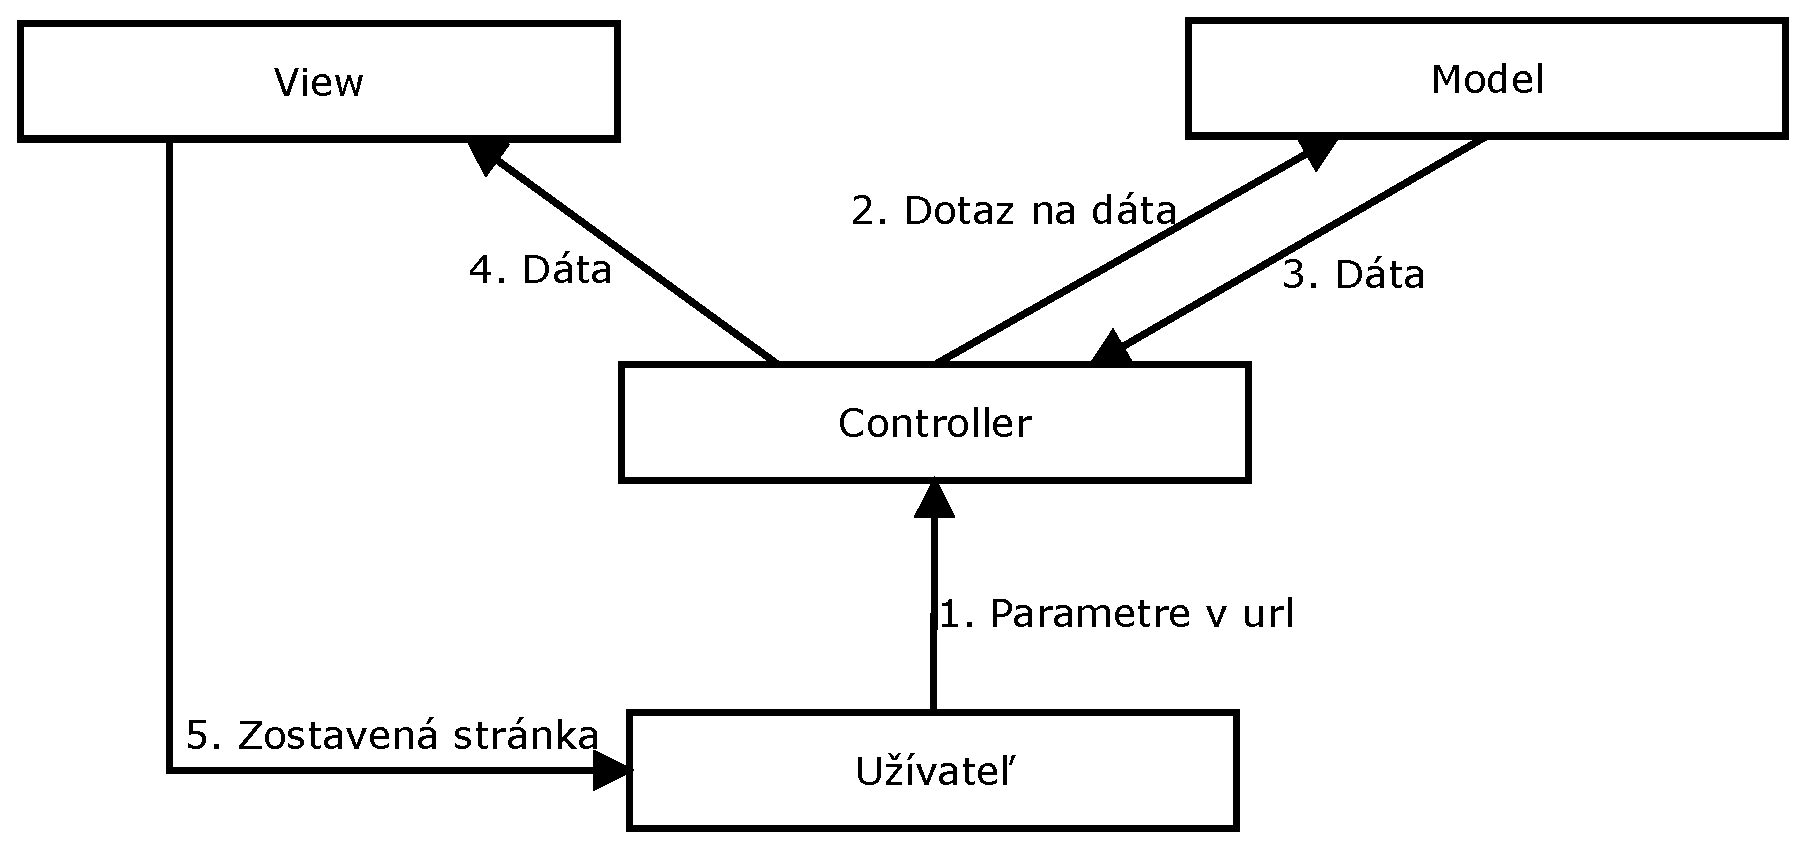
\includegraphics[scale=0.40]{fig/mvc.eps}
  \caption{Príklad MVC}
  \label{fig:mvc}
\end{figure}

\subsection{Nette}
\label{sec:nette}
PHP je síce samo o sebe mocný programovací jazyk, ale v prípade zvolenia čistého PHP, by programátor musel riešiť veľké množstvo vecí, ktoré niekto v minulosti už dávno efektívnejšie vyriešil. Okrem toho by si programátor musel dávať veľký pozor a ošetrovať početné množstvo bezpečnostných rizík. Kvôli týmto veciam bol pre účel práce vybraný aplikačný rámec Nette.

Nette je rámec napísaný v PHP5, ktorý sa zameriava na pohodlnejšie a rýchlejšie programovanie webových aplikácií a elimináciu bezpečnostných rizík. Podporuje MVC a OOP. Z veľkej časti je založený na vytváraní znovu použiteľných komponentov. K Nette patrí aj šablónovací systém Latte, ktorý zapuzdruje PHP v HTML súboroch do špeciálnych Latte makier a tým eliminuje bezpečnostné riziká. Tracy a Tester zase slúžia na hľadanie a odlaďovanie chýb. Pôvodným autorom je David Grundl, ale v súčasnosti sa o rozvoj rámcu stará Nette Foundation. Je ponúkaný pod licenciou GNU GPL a licenciou Nette (obdoba BSD licencie). Rámec sa teší veľkej obľube a taktiež početnej komunite v Čechách a na Slovensku. Minimálne požiadavky, pre správnu funkčnosť rámca, sa vyžaduje PHP verzie 5.3.1 a vyššej. Všetky požiadavky je možné overiť oficiálnym checker.php skriptom.

\section{Databázová časť}
\label{sec:databaza}
Databáza, ako prostriedok pre uloženie dát, bola zvolená hlavne kvôli vlastnosti ACID\footnote{atomickosť, konzistencia, izolovanosť a trvácnosť} a pre prístup viacerých užívateľov k databázy súčasne. Okrem iného, databázy šetria pamäťové miesto tým, že pri dobrom návrhu sa v databázy nenachádzajú redundantné dáta. Manipulácia s dátami je pomerne rýchla, pretože sa do medzi pamäte neukladá celá databáza. Nad databázou sa dajú vykonávať zložité dotazy a spájať dáta z viacerých tabuliek.  Na výber boli rôzne alternatívy ako napríklad PL/SQL, T-SQL alebo vybraný MySQL.   

\subsection{MySQL}
\label{sec:mysql}
MySQL je otvorený, viac užívateľský SQL relačný databázový server, ktorý je implementovaný vo viacerých programovacích a hlavne serverových jazykoch, napríklad v skriptovacom jazyku PHP. Je to databázový relačný systém, teda každá databáza v MySQL je tvorená z jednej alebo viacerých tabuliek, ktoré majú riadky a stĺpce. Riadky udávajú jednotlivé záznamy, stĺpce zase dátové typy jednotlivých záznamov. Práca s takouto databázou je vykonávaná pomocou takzvaných dotazov.

\section{Klientská časť}
\label{sec:klient}
Klientská časť pokrýva všetko to, čo je zobrazené užívateľovi. Teda v tomto prípade je myslená kompletná stránka, ktorej zostavovanie sa dialo z väčšej miery na servery. Aby boli informácie určené pre užívateľa zobrazené v nejakej prijateľnej a užívateľsky prívetivej podobe, tak sa vyžaduje okrem značkovacieho jazyka HTML použiť aj CSS kaskádové štýly. Keďže moderná prezentácia informácií na webových portáloch vyžaduje aj určitú ľahkosť a dynamiku, tak k tomuto účelu bol použitý celosvetovo rozšírený programovací jazyk Javascript.

\subsection{HTML}
\label{sec:html}
Hyper Text Markup Language je značkovací jazyk určený pre popis webových dokumentov, hlavne webových stránok. Najprv bol iba veľmi jednoduchá podmnožina jazyka SGML\footnote{Standard Generalized Markup Language}, ale neskôr sa z neho vyvinul samostatný štandard. HTML dokument sa popisuje pomocou HTML tagov. Každý typ HTML tagu slúži na popísanie odlišného typu obsahu dokumentu.  

V minulosti sa HTML používal na definovanie štruktúry dokumentu a aj jeho výzoru. V súčasnej dobe je HTML určené iba na zmienenú definíciu štruktúry.

\subsection{CSS}
\label{sec:css}
Kvôli tomu, že HTML sa začalo používať iba na definovanie štruktúry dokumentu a nie jeho výzoru, bol vyvinutí Cascading Style Sheets. CSS popisuje ako budú HTML tagy zobrazené na obrazovke, papieri, alebo inom médiu. CSS šetrí veľa času tým, že môže popisovať rozmiestnenie viacerých webových stránok naraz.

\subsection{Javascript}
\label{sec:javascript}
Javascript je skriptovací, prototypovo založený jazyk, ktorý sa v súčasnosti používa hlavne pri tvorbe dynamických webových prezentácií a webových stránok. Javascript beží na klientskej strane webu. Je spúšťaný väčšinou vo webových prehliadačoch. V súčasnosti Javascript podporuje väčšina webových prehliadačov a je najpoužívanejší skriptovací jazyk používaný na klientskej strane.

Bola by chyba myslieť si, že Javascript svoje uplatnenie pri tvorbe webov má iba na strane klienta. Javascript je naozaj všestranný jazyk a svoje uplatnenie nájde aj na servery napríklad v podobe Node.js. Pre účely tejto práce je avšak použitý klasický klientský Javascript spúšťaný vo webovom prehliadači.

\subsection{JQuery}
\label{sec:jquery}
JQuery je ľahká a rýchla Javascriptová knižnica, ktorej hlavným cieľom je, aby bolo použitie Javascriptu na webových stránkach omnoho jednoduchšie. Taktiež zjednodušuje komplikované veci Javascriptu, ako AJAX volania a manipuláciu s DOM. Okrem toho obsahuje metódy na manipuláciu s CSS, HTML udalosti, efekty a animácie a ďalšie nápomocné programy. Je rozšíriteľná pomocou pluginov a na väčšinu známych vecí už existuje JQuery plugin. Knižnica zároveň rieši tzv. cross-browser problémy, kedy jedna vec sa môže v rôznych prehliadačoch správať odlišne.

Je to najobľúbenejšia a najrozšírenejšia Javascriptová knižnica, čomu dáva za pravdu nielen početná komunita okolo, ale aj to, že je využívaná najväčšími firmami ako Google, či Microsoft.

\subsection{Bootstrap}
\label{sec:bootstrap}
Bootstrap je frontendový aplikačný rámec pre rýchle a ľahké vyvíjanie responzívnych webových stránok. Obsahuje predpripravené dizajnérske typografické šablóny založené na HTML a CSS. Hodí sa predovšetkým na prototypovanie, hlavne kvôli značnej neoriginalite vytvorených stránok, keďže väčšina stránok založená na tomto rámci vypadá veľmi podobne. Na druhú stranu, jednoduchými modifikáciami si môže skúsený dizajnér upraviť Bootstrap k svojmu obrazu.   

\subsection{Chart.js}
\label{sec:chartjs}
Chart.js je ľahká Javascriptová knižnica, pomocou ktorej je tvorba grafov z daných dát veľmi jednoduchá. Na zobrazovanie grafov používa HTML tag <canvas > do ktorého sa grafy vykresľujú. Na výber je z 6 najbežnejších typov grafov. Takto vytvorené grafy sú plne responzívne, takže môžu byť správne zobrazené, ako na stolných počítačoch s veľkou obrazovkou, tak aj na malých mobilných zariadeniach.

\section{API}
\label{sec:api}
API je v tomto prípade myslené, ako knižnica, pomocou ktorej vývojári hier pristupujú k funkciám webovej platformy. Knižnica je implementovaná v Javascripte a k funkciám platformy, ktoré sú implementované na servery sa pristupuje pomocou dotazovaním technológiou AJAX.

\subsection{AJAX}
\label{sec:ajax}
Asynchronous Javascript and XML je súhrnné označenie technológií, ktoré umožňujú meniť obsah webových stránok bez nutnosti znovu načítania celej stránky zo servera. Hlavná výhoda spočíva v tom, že sa prenáša značne menšie množstvo dát. AJAX nie je samostatný programovací jazyk, ani technológia sama o sebe, ako by sa mohlo zdať. Je to skôr kombinácia niekoľkých prvkov. Je založený na internetových štandardoch. Používa kombináciu HMLHttpRequest pre získanie dát zo servera a Javascript/DOM pre zobrazenie a použitie dát.
\begin{figure}[h]
  \centering
  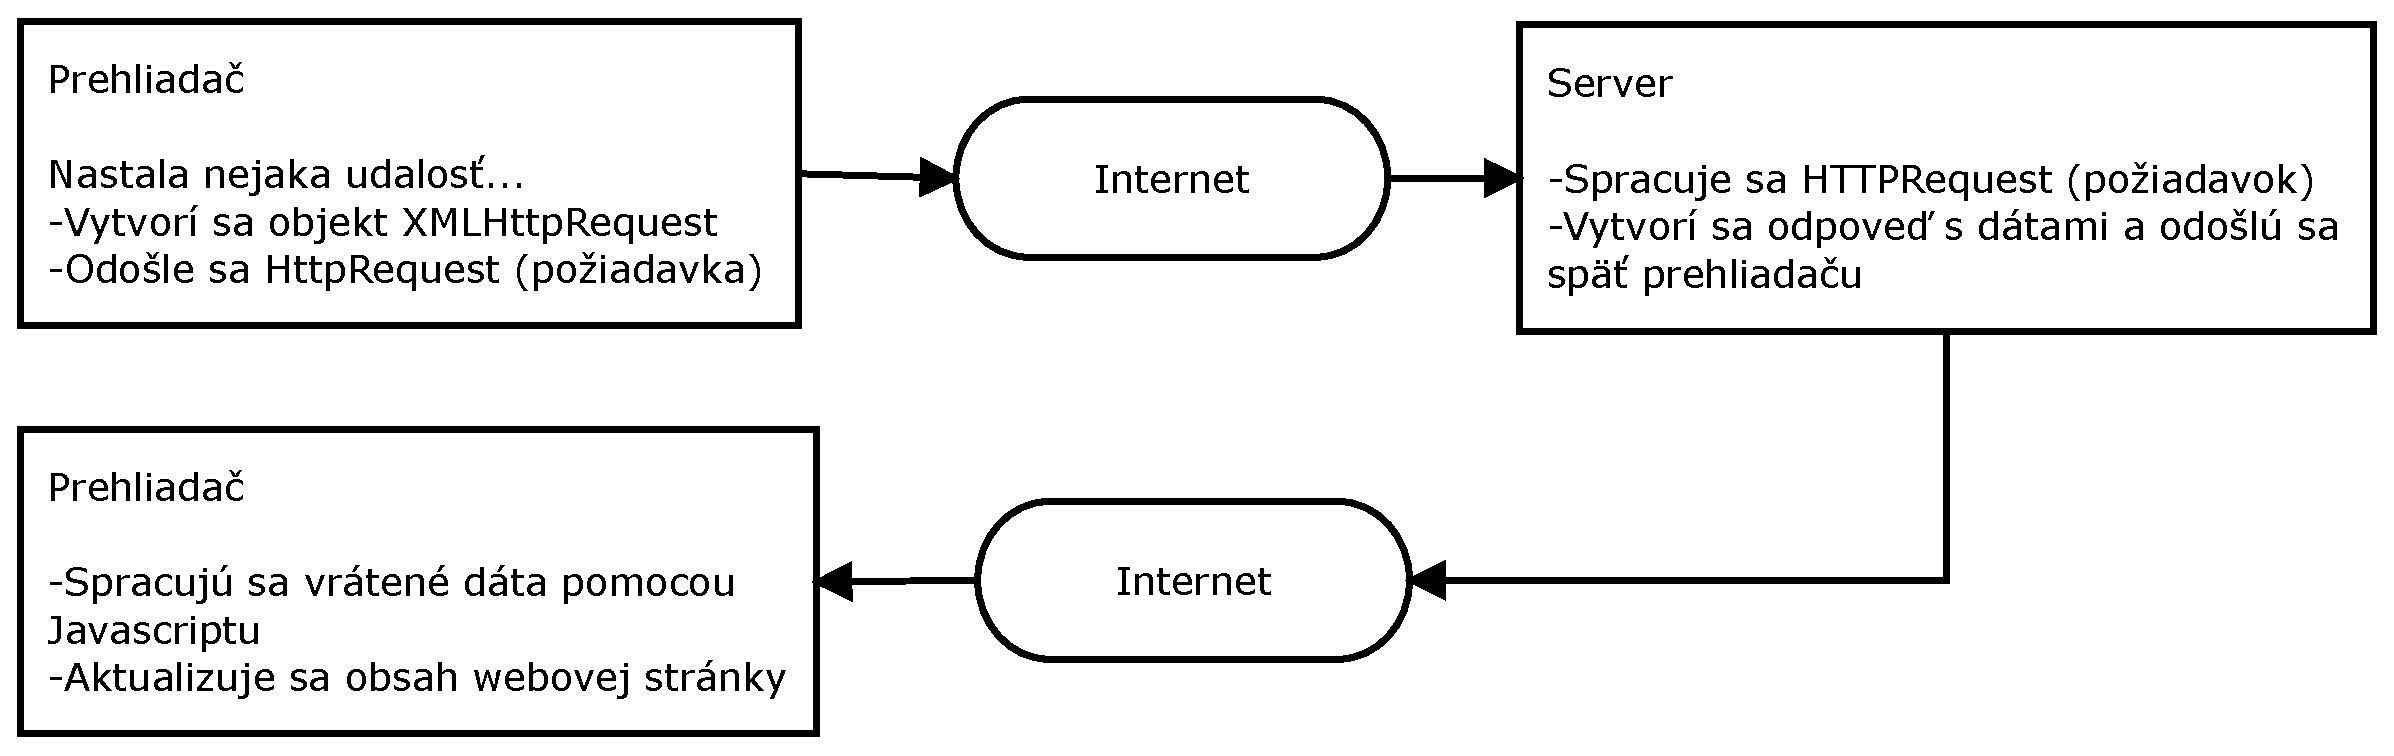
\includegraphics[scale=0.40]{fig/ajax.eps}
  \caption{Neblokujúca komunikácia so serverom pomocou AJAXu}
  \label{fig:ajax}
\end{figure}

\subsection{CORS}
\label{sec:cors}
Klasický Javascript je limitovaný tzv. Same origin policy. Z toho dôvodu nie je možné prijímať odpovede na dotazy z domény inej, ako je doména z ktorej bola požiadavka vyslaná.

Tento známy, hore popísaný problém rieši Cross-origin resource sharing. CORS je vlastne mechanizmus, ktorý povoľuje zakázané zdroje na webovej stránke, a tak je možné prijímať odpovede na požiadavky z inej domény, ako z domény z ktorej zdroje pochádzajú. Pre použitie tohto mechanizmu musí nastať zmena pri tvorbe požiadavku na klientovi a tiež je treba povoliť CORS na servery. Prehliadač musí posielať nastavenie Origin: doména v HTTP hlavičke. Na servery zase musí byť nastavené povolenie Acces-Control-Allow-Origin: doména, alebo * pre povolenie všetkých domén.

\section{Hra}
\label{sec:hra}
Pre demonštračnú hru sa ponúkalo buďto použiť klasický Javascript, čo ale nie je príliš rozšírená forma tvorby Javascript/HTML5 hier, alebo použiť jeden z početného množstva aplikačných rámcov, ktoré sú určené špeciálne na tvorbu hier. Na výber bol Ease.js, Tree.js, Panda.js, melon.js, Kiwi.js, alebo Phaser.js a mnoho ďalších. Bol vybraný Phaser.js, pretože to je jeden z najpoužívanejších a najbežnejších Javascriptových rámcov určených pre programovanie hier, o čom svedčí hlavne početná komunita okolo tohto rámca a fakt, že aj mnohé firmy z oblasti herného biznisu, ako Boostermedia, pracujú práve s týmto rámcom. 

\subsection{Phaser}
\label{sec:phaser}
Phaser je Javascriptový aplikačný rámec určený špeciálne pre tvorbu hier, ako desktopových, tak aj mobilných. Je založený na renderovacom rámci pixi.js. Phaser je ľahko osvojiteľný, rýchly, je ponúkaný zadarmo a má otvorený kód. Podporuje canvas a zároveň aj webgl. Obsahuje veľké množstvo predpripravených funkcií. Tieto funkcie sú spracované tak, aby ich použitie bolo jednoduché. Príkladom môže byť stavaný preloader, fyzika, animácie, častice, rôzne módy prispôsobenia veľkosti obrazovky a iné.  

\chapter{Analýza existujúcich riešení}
\label{chap:analyza}
V tejto kapitole budú predstavené konkurenčné, existujúce riešenia určené pre iné platformy, ako je platforma, pre ktorú je riešenie tejto práce určené. 

%%%%%%%%%%%%%%%%%%%%%%%%%%%%%%%%%%%%%%%%%%%%%%%

\section{Steam}
Steam je herná platforma od spoločnosti Valve Corporation určená predovšetkým k digitálne distribúcií hier a vytvoreniu komunity hráčov daných hier. Steam klient je podporovaný na rôznych platformách. Na počiatku podporoval iba platformu Windows, neskôr svoje pôsobenie rozšíril na platformu Mac a nakoniec na Linuxové distribúcie. Pochopitelne nie všetky hry nachádzajúce sa na steam platforme sú hrateľné vo všetkých operačných systémoch. Moemntálne samotná platforma obsahuje viac ako 3500 hier a teší sa početnej komunite hráčov. 

Steam pre vývojárov hier, ktoré boli schválené komunitou steam greenlight pre možnosť distribúcie hry na platforme, ponúka svoje Steamworks API. Steamworks API dovoluje vývojárom hier integrovať rôzne funkcie ako štatistiky, odmeny, autentifikácia, tvorba zápasov, peer-to-peer networking, steam cloud úložisko, valve anticheat, hlasový chat a v neposlednej rade aj DRM.
\begin{figure}[h]
  \centering
  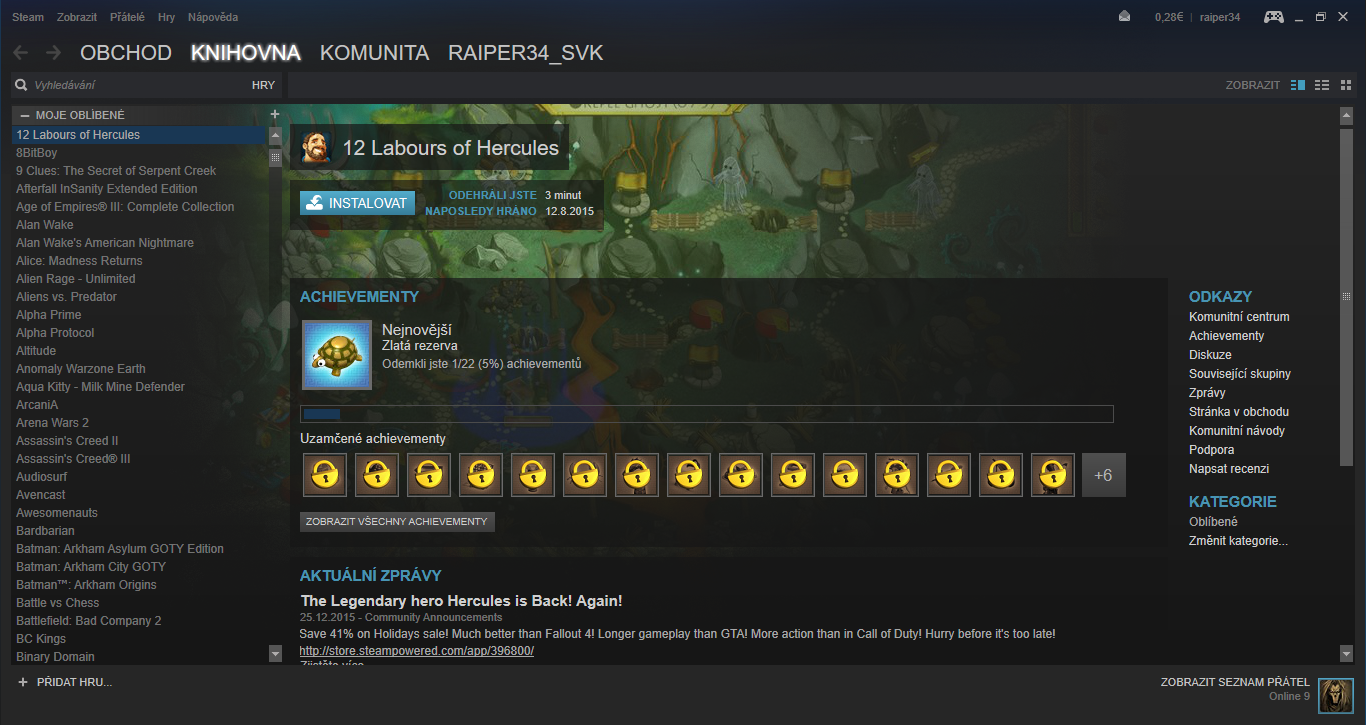
\includegraphics[scale=0.27]{fig/steam.png}
  \caption{Ukážka steam klienta na Windows}
  \label{fig:steam}
\end{figure}

\section{Google Play Game Services}
Po predstavení operačného systému Android vyvinul Google svoj internetový obchod Google play, ktorý ponúka nielen aplikácie a hry pre android, ale po novom aj knihy hudbu a filmy. Vývojári momentálne môžu získať prústup na publikovanie aplikácií  v tomto obchode za 20USD, pričom reálne nie sú limitovaný počtom aplikácií a ani kvalitou.  

Okrem toho, Google povoľuje vyvojárom hier integrovať do svojich hier svoje Play Game Services API. Zprvu bolo API limitované iba na Android hry, momentláne avšak podporuje aj webové. Pred samotným použitím API si vývojár musí najprv definovať hru v Google Play Developer Console a poprípade ďalšie doplnkové funkcie. API ponúka možnosťi použitia odmien, score tabuliek, multiplayeru, uloženia dát v cloude, udalosti a úlohy a iné. 
\begin{figure}[h]
  \centering
  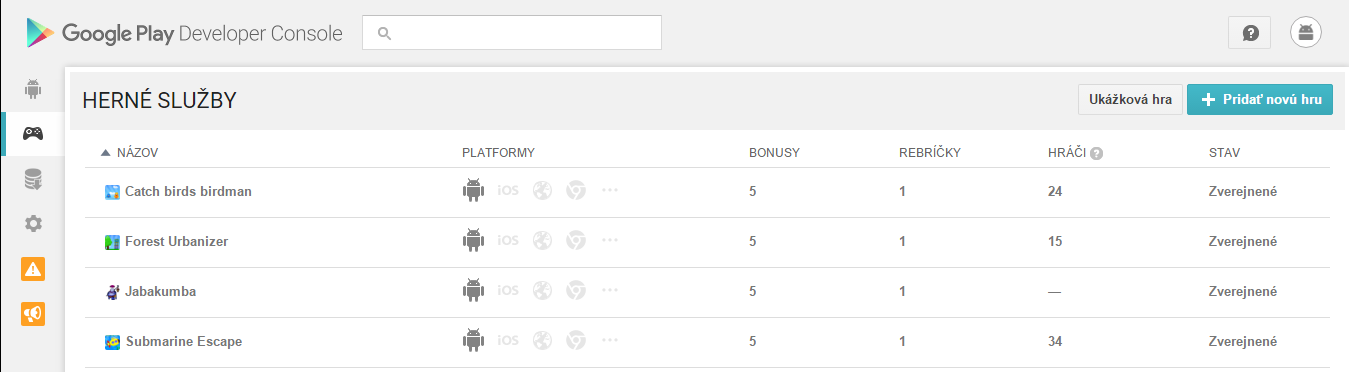
\includegraphics[scale=0.32]{fig/google-play.png}
  \caption{Ukážka Google Play Developer Console  - zoznam existujúcich hier}
  \label{fig:google-play}
\end{figure}

\section{Apple Game Center}
Rovnako ako Google má pre Android svoj internetový obchod a aplikáciami, tak aj Apple má svoj App Store. Narozdiel od Google play, vývojár pre prístup do App Store musí platiť ročne buď 99 USD za Apple Developer Program, alebo 299 USD za Apple Developer Enterprise Program. Viac informácií je, ako aj rozdiely v týchto programoch je možné nájsť na ích officialnej stránke. 

Taktiež Apple ponúka svoje Game Center API. API je integrovateľné do iOS hier a taktiež do OS X. Game Center umožnuje integrovať score tabuľky, odmeny, pozývanie priateľov do hry a spúštanie multiplayer hier pomocou systému automatického vytvárania hier.

\section{Clay.io}
Clay.io je webový projekt zameraný na Javascriptové/HTML5 hry. Vytvoril ho v roku 2012 Austin Hallock. Z prvu bol tento projekt rovnomerne orientovaný na vývojárov hier a aj hráčov týchto hier. Platforma neobsahovala žiadne kvalitatívne obmedzenia čo sa týka uverejnovania hier a jej služby boli zadarmo. Bolo možné do hry integrovať vlastné API, ktoré zprístupňovalo score tabuľky, odmeny, cloud úložisko dát, cross promotion, reklamy tretích strán. Okrem toho na základe už vložených informácií Clay.io dokázalo generovať rôzne konfiguračné súbory pre webové obchody ako Chrome web store alebo Mozzila marketplace a iné. Začiatkom roka 2015 sa avšak situácia zmenila a Clay.io sa uzavrelo. Začalo sa orientovať na vyššiu kvalitu hier a k API už môžu pristuovať iba oprávený schválený vývojári a publikovať tieto hry s integrovaným API je možné iba na webe Clay.io a v špeciálnej Clay.io aplikácií, ktorá je určená pre Android.    

\section{Ostatné}
Pre webové hry postavené na technológií Flash existovalo a stále existuje hneď niekoľko herných portálov určených predovšetkým pre hráčov, ktoré ponúkajú taktiež vývojárom možnosť integrovať rôzne služby webového portálu do hry. Príkladom môže byť zaniknutý Mochimedia, alebo stále existujúce herné webové portále Newgrounds.com, Gamejolt.com, alebo Kongregate.com. Nevýhodou týchto portálov je to, že použitie ich API, je často limitované iba využitie na danom webovom portáli. Všetky zmienené portáli ponúkali, alebo stále ponúkajú obdobné funkcie API, ako tomu bolo v predchádzajúcich kapitolách, teda highscore tabuľky, odmeny, úložisko v cloude, ochrana hry, udalosti a niektoré dokonca reklamy, alebo chatovacie miestnosti.
\begin{figure}[h]
  \centering
  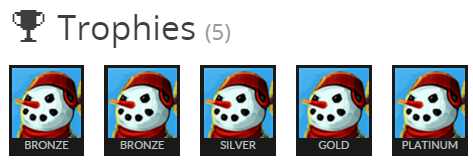
\includegraphics[scale=0.5]{fig/odmeny2.png}
  \caption{Ukážka odmien na stránke Gamejolt.com}
  \label{fig:odmeny}
\end{figure}

\chapter{Návrh riešenia}
\label{chap:navrh}
Táto kapitola popisuje návrh riešenia tejto bakalárskej práce. Najprv pojednáva o analýze požiadavkov na komponenty, ktoré sú zahrnuté v API a na celkovú štruktúru webovej platformy. Ďalej popisuje návrh databáze a je predstavený jej konceptuálny model. Ďalšia podkapitola je venovaná návrhu rozhrania webového portálu, jeho časti určenej pre hráčov, časti určenej pre vývojárov a aj časti pre administrátorov. A nakoniec je predstavený návrh jednoduchej HTML5 hry, ktorá má za úlohu demonštrovať funkcie API.  

\section{Analýza požiadavkov na komponenty}
Požiadavky na komponenty čiastočne vychádzajú z predchádzajúcej kapitoli o Analýze už existuúcich riešení. Boli vybrané komponenty z daných existujúcich riešení také, ktoré sa najviac opakovali v daných službách, a ktoré boli reálne použiteľné na webovej platforme. Okrem toho bol zostavený orientačný doplňujúci dotazník, cielený práve na vývojárov hier a špeciálne na vývojárov webových html5 hier. Dáta boli zberané na fórach, kde sa združujú vývojári takýchto hier a v skupinách sociálnych skupín, ktoré taktiež obsahujú takýchto ľudí. V dotazníku odpovedalo viac ako 100 ľudí a týto ľudia mali vybrať 3 komponenty, ktoré pokľadajú pre seba ako vývojárov za najužitečnejšiu, pritom bolo jendo z akého hladiska, či z toho hladiska toho, že komponenta má obohacovať hru napríklad o tabuľku skóre, či odmeny a tak jej pridávať na atraktivite, alebo naopak má slúžiť vývojárovi ako napríklad štatistiky prístupov, alebo kontrola domény, na ktorej sa daná hra nachádza.   Výsledky môžete vidieť na obrázku. Dáta slúžia iba pre predstavu, čo najviac vývojárom chýba, alebo naopak, ktoré komponenty z vymenúvaných pokľadajú z ích hľadiska za najdôležitejšie, najprínosnejšie.
\begin{figure}[h]
  \centering
  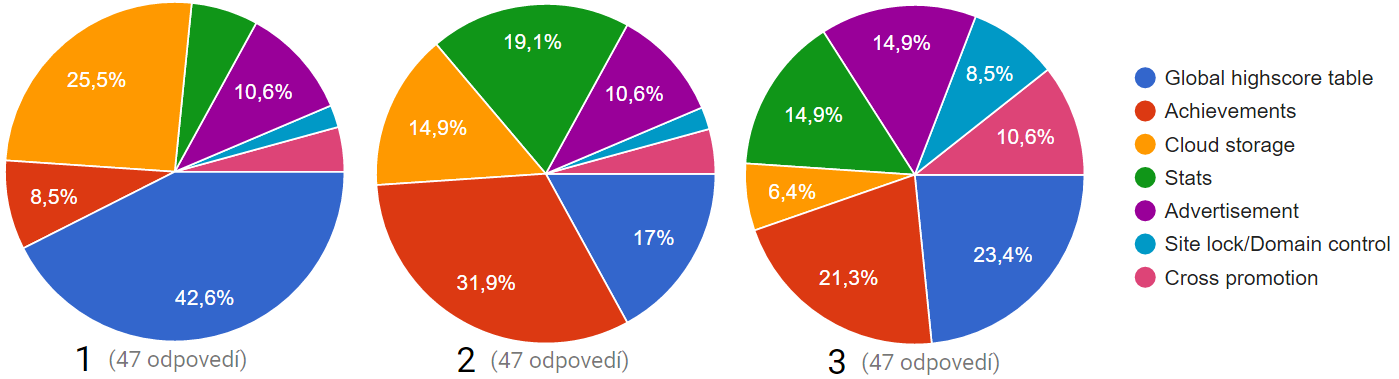
\includegraphics[scale=0.7]{fig/graf-dotazniku.png}
  \caption{Výsledky dotazníku}
  \label{fig:dotaznik}
\end{figure}

Na základe tohto dotazníku, ale predovšetkým na základe analýzy už existujúccih riešení bola vybraná nasledujúca množina komponent.
\begin{enumerate}
\item Tabuľky skóre
\item Odmeny
\item Kontrola domén
\item Štatistiky prístupov
\item Úložisko v cloude
\end{enumerate}
Niektoré komponenty neboli vybrané z dôvodu, že neboli pokladané vývojármi za až tak podstatné (napríklad cross-promotion), alebo sa nehodili k danému projektu (napríklad chat, ktorý by v hre na mobilných zariadeniach s nie až tak veľkými obrazovkami, mohol byť viac na obtiaž, než k úžitku). Ďalšia komponenta, s ktorou sa v tomto projekte nepočíta, aj keď v dotazníku bola táto možnosť celkom vyberaná, je integrácia reklám do hry. Takáto komponenta by bola nad rámec tejto práce a muselo by sa okolo nej riešiť niekoľko ďalších vecí, ako získanie inzerentov, správa reklamných kampaní a ďalšie z väčšej miery netechnické veci.

\section{Návrh webovej platformy}
Návrh webovej platformy bol vypracovávaný po analýze existujúcich herných platforiem, klientov a webových portáloch, ktoré sú čiastočne uvedené v kapitole 3. V prvom rade bolo treba premyslieť, k čomu všetkomu daná webová platformu by mala slúžiť, čo všetko by na nej malo byť realizovateľné, aké možnosti by ponúkala pre vývojárov hier a aké možnosti zase pre hráčov týchto hier. 

Tento návrh, toho, čo všetko môže daný užívateľ so svojoou rolou na portáli vykonávať bol spracovaný pomocou Use Case Diagramu (Diagramu prípadov užitia) ďalej iba UCD, ktorý zobrazuje chovanie systému, tak ako ho vidí užívateľ. Účelom tohto diagramu je popísať funkcionalitu systému, teda čo sa od systému očakáva. Diagram hovorí o tom, čo má systém, v tomto prípade naša webová platforma vedieť, ale nehovcorí o tom, ako sa to bude vykonávať. V UCD sa skladá z prípadov užiatia (Use Case), aktérov (Actor) a vzťahov medzi nimi. Prípad užitia je sada niekoľkých akcií, ktoré vedú k dosiahnutiu určitého cieľa. Aktér je roľa, ktorá komunikuje s jednotlivými prípadmi užitia. Zjednodušene povedané UCD je diagram, ktorý zobrazuje to, čo všetko daná užívateľská roľa môže v systéme vykonávať. Na obrázku môžete vidieť naľavo aktéra a napravo prípad užitia. 
\begin{figure}[h]
  \centering
  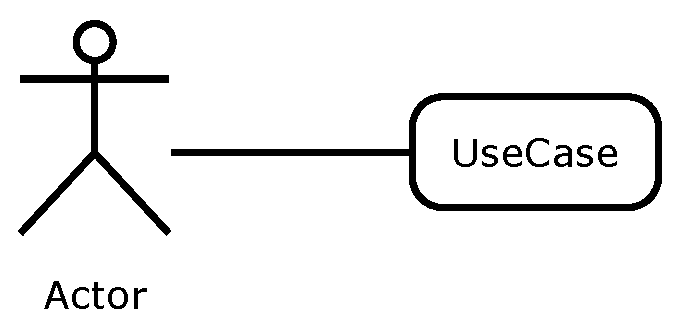
\includegraphics[scale=0.4]{fig/ucd.eps}
  \caption{Use Case Diagram, naľavo aktér, napravo prípad užitia}
  \label{fig:ucd}
\end{figure}

Prvou roľou, ktorou sa užívateľ stáva po príchode na webovú platfomu je roľa neprihláseného návštevníka. Prirodzene neprihlásený, často ešte nezaregistrovaný návštevník musí mať obmedzenú množinu toho, čo môže na danej stránke vykonávať. V prípade tejto bakalárskej práce môže byť neprihlásený užívateľ napríklad hráč, ktorý sa ešte nezaregistroval, alebo sa z nejakého dôvodu nechce registrovať. Na portál prišiel vyložene !zabiť! čas, highscore tabuľky ho nemotivujú k súťaženiu s ostatnými hráčmi a ani odmeny sa mu nijak zaujímavo nevidia. Keďže platforma by mala byť optimalizovaná pre prenosné zariadenia ako mobily a tablety, tak to môže byť hráč s mobilným zariadením čakajúci napríklad v ordinácií lekára, alebo čakajúci na autobusovej zastávke. Takýto hráč teda potrebuje jediné, zobraziť zoznam hier, aby si vybral hru, tkroú chce hrať, poprípade filtrovať zoznam hier podľa nejakých kategórií, ako napríklad žánru... Po vybraní hry si chce prečítať nejaké základné informácie o hre, inštrukcie ako hru ovládať a v neposlendom rade náhľady,a elbo iné grafické matertiály, pochádzajúce najlepšei priamo z danej hry. Po tom všetkom chce samozrejme daný hráč hrať samotnú hru umiestnenú na portáli. Neprihláseným návštevníkom môže byť avšak aj hráč, ktorý sa chce na daný portál prihlásiť, poprípade sa zaregistrovať a mať tak možnosť využívať všetku funkcionalitu daného portálu  určenú pre roľu prihláseného hráča. Poslendým príkladom, ktorý bude uvedený ako neprihlásený návštevník je napríklad, užívateľ, tkroý che na tomto portáli získať roľu vývojjára hry a mať tak možnosť sa podielať na tvorbe herného obsahu, alebo využívať iné funckie určené vývojárom. Diagram prípadov užitia, ktorý zhrnuje tento odsek je na obrázku.
\begin{figure}[h]
  \centering
  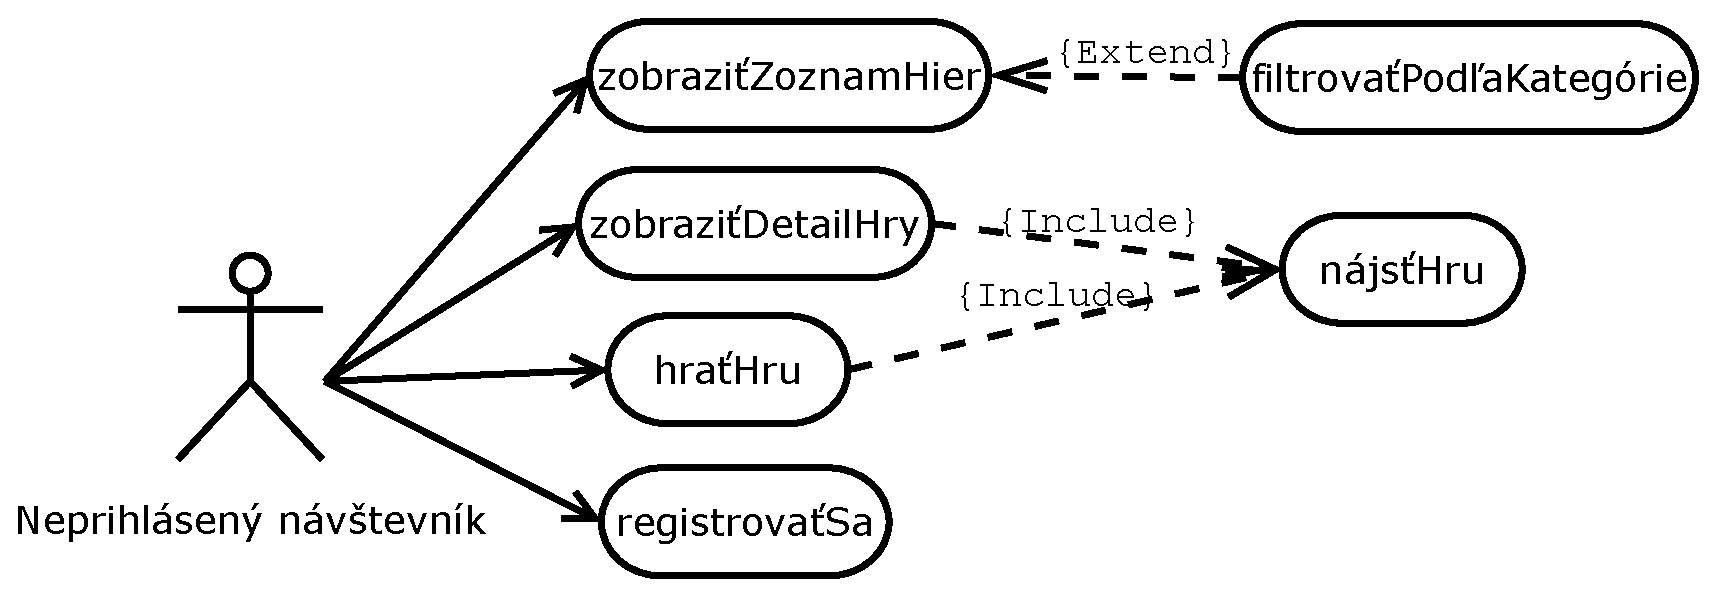
\includegraphics[scale=0.4]{fig/ucd-neprihlaseny.eps}
  \caption{Use Case Diagram neprihláseného užívateľa}
  \label{fig:ucdneprihlaseny}
\end{figure}

V poradí druhou roľou kterou sa užívateľ môže stať v rámci systému je roľa prihláseného hráča. Nperihlásený návštevník sa prihláseným hráčom stáva od chvíľe kedy sa prihlási k svoju účtu hráča.  Prihlásený hráč môže vykonávať na portáli všetky akcie, ktoré môže vykonávať roľa neprihláseného návšetvníka, a k tomu ešte môže vykonávať ďalšie akcie, na ktoré je potrebné byť prihlásený. Prihlásený hráč môže hrať hry pod svojim účtom a tým pádom získavať v danej hre odmeny a umiestnovať sa v score tabuľkách najlepších hráčov a tým nepriamo súťažiť s ďalšími prihlásenými hráčmi. Okrem toho prihlásený hráč má možnosť číselne ohodnotiť hru, alebo zdielať svoje pocity z hry s ostatnými publikovaním svojho komentáru na stránke s hrou. Hráč by mal mať možnosť tiež prezerať si svoj hráčský profil a profil ostatných hráčov. Usa case diagram, ktorý popisuje akcie prihláseného hráča môžete vidieť na obrázku.
\begin{figure}[h]
  \centering
  \includegraphics[scale=0.4]{fig/ucd-prihlasenyhrac.eps}
  \caption{Use Case Diagram neprihláseného užívateľa}
  \label{fig:ucdprihlasenyhrac}
\end{figure}

\section{Návrh databáze}

\section{Návrh API}

\section{Návrh Hry}

\section{Znovupoužiteľné komponenty}
todo

\subsection{Odmeny}
todo

\subsection{Tabuľky najlepších hráčov}
todo

\subsection{Štatistiky}
todo

\subsection{Úložisko v cloude}
todo

\chapter{Implementácia}
\label{chap:implementacia}
todo

\chapter{Testovanie}
\label{chap:testovanie}
todo

\chapter{Záver}
\label{chap:zaver}
todo












%=========================================================================
